\documentclass{beamer}

\usepackage{fontspec}
\usepackage{xeCJK}
\setCJKmainfont{DFFN_R3.TTC}
\XeTeXlinebreaklocale "zh"
\XeTeXlinebreakskip = 0pt plus 1pt
\linespread{1.3}
\allowdisplaybreaks

\newcommand{\weib}{\CJKfamily{weib}}
\newcommand{\hkss}{\CJKfamily{hkss}}
\newcommand{\hksy}{\CJKfamily{hksy}}
\newcommand{\lth}{\CJKfamily{lth}}
\usepackage{color}
\usepackage{booktabs}
\usepackage{tabularx}
\usepackage{caption}
\usepackage{tikz}
\usepackage{verbatim}
\usepackage{pgfplotstable}
\pgfplotsset{width=12cm}
\pgfplotsset{height=7cm}
\pgfplotsset{compat=1.13}

\usetheme{EastLansing}
\usetikzlibrary{positioning}
\useinnertheme{rectangles}
\usefonttheme{professionalfonts}

\newcommand{\lw}{0.8mm}
\setbeamercovered{transparent}


%\AtBeginSection[]
%{
  %\begin{frame}<beamer>
	%\frametitle{報告大綱}
	%%\frametitle{RoadMap}
    %\tableofcontents[currentsection]
  %\end{frame}
%}

\title{More on Adversarial Attack/Defense}
%\subtitle{\textcolor[rgb]{0.00,0.50,1.00}{{Adversarial Attack/Defense in Machine Learning}}}
\author{徐瑞陽}
\date{2019/05/16}
\begin{document}



\begin{frame}
\maketitle
\end{frame}

\begin{frame}
\frametitle{Outline}
\tableofcontents
\end{frame}

\begin{frame}{Recap: Optimization View on Adversarial Robustness}
  \begin{block}{Objective}
    \[ \min_\theta \mathbb{E}_{(x,y) \sim \mathcal{D}}[\max_{\delta \sim \mathcal{S}}L(x+\delta,y|\theta)]\]
  \end{block}
  \begin{itemize}
    \item $\mathcal{S}$: allowed pertubations of adversary
    \item $\theta$: weights of classifier model
    \item $\mathcal{D}$: data distribution
    \item $L(\cdot)$: loss function
  \end{itemize}
\end{frame}

\section{Trade-off Between Standard Accuracy \& Adversarial Robustness}

\begin{frame}
    \center \LARGE{Why not just train with all adversarial samples?}
\end{frame}

\begin{frame}
    \center \LARGE{Is adversarial robustness FREE?}
\end{frame}

\begin{frame}{Trade-off of Adversarial Robustness}
  \begin{itemize}
    \item More training time
    \item \textbf{Generalization accuracy drops} 
  \end{itemize}
\end{frame}

\begin{frame}{Robustness May Be At Odds With Accuracy}
  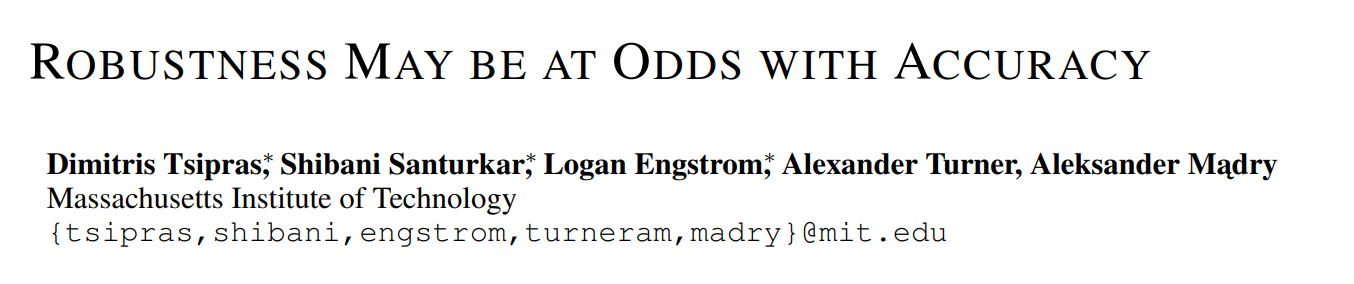
\includegraphics[width=\textwidth]{fig/p2/title.png}
  \center ICLR 2019
\end{frame}

\begin{frame}{Example: Binary Classification Task}
  Consider binary classification task, $(x,y) \sim \mathcal{D}$ as follows
  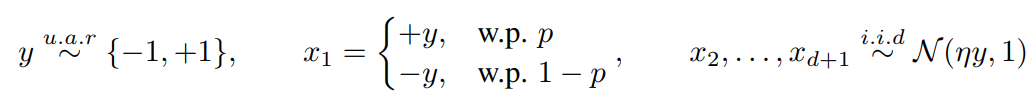
\includegraphics[width=\textwidth]{fig/cls.png}
  We choose $\eta$ be large enough to separate these 2 distributions ($\eta = \Theta(1/\sqrt{d})$)  

  \begin{itemize}
    \item $x_1$ is \textit{moderately correlated} with the label (say, $p=0.8$)
    \item $x_2 \sim x_{d+1}$ is \textit{very weakly correlated} with the label ($p = 0.5 + \epsilon$)
  \end{itemize}
\end{frame}

\begin{frame}{Standard Classification is Easy}
  \begin{block}{Observation}
    Although each $x_2 \sim x_{d+1}$ feature is weakly correlated, the average of them is \textit{highly correlated} 
  \end{block}
  Consider a linear classifier $f_{avg}$

  \[
    f_{avg}(x) := \texttt{sgn}(w_{unif}^T x), \quad \text{where} \, w_{unif}:= \Big[0,\frac{1}{d},\cdots,\frac{1}{d}\Big]
  \]

\end{frame}

\begin{frame}{Standard Classification is Easy (cont.)}
  \begin{block}{Linear classifier}
  \[
    f_{avg}(x) := \texttt{sgn}(w_{unif}^T x), \quad \text{where} \, w_{unif}:= \Big[0,\frac{1}{d},\cdots,\frac{1}{d}\Big]
  \]
  \end{block}
  Standard accuracy is 
    \begin{align*}
      \Pr[f_{avg}(x) = y] &= \Pr[\texttt{sgn}(w_{unif}^T x) = y]  \\
                          &= \Pr \Big[\frac{y}{d}\sum_{i=1}^d \mathcal{N}(\eta y,1) > 0 \Big] \\
                          &= \Pr \Big[\mathcal{N}(\eta,\frac{1}{d}) > 0 \Big]
    \end{align*}

  which is $> 99\%$ when $\eta \geq 3 / \sqrt{d}$
\end{frame}

\begin{frame}{Adversarially Robust Classification}
  Consider moderate pertubation $\delta$, which $L_\infty \leq \epsilon = 2 \eta$...\\
  Those correlated features become \textbf{anti-correlated}

  Adversarial accuracy is
    \begin{align*}
      \Pr[\texttt{sgn}(x + \delta) = y] &= \Pr \Big[\frac{y}{d}\sum_{i=1}^d \mathcal{N}(-\eta y,1) > 0 \Big] \\
                                &= \Pr \Big[\mathcal{N}(-\eta,\frac{1}{d}) > 0 \Big]
    \end{align*}

  The classifier derived before cannot get adversarial accuracy better than $1\%$
\end{frame}

\begin{frame}{Some Lessons}
  \begin{itemize}
    \item For standard classifier, any feature which is weakly correlated is useful, so the model will exploit them
    \item On the other hand, adversary can also simply exploit these features by a moderate $\epsilon$ (where $\epsilon = \mathcal{O}(1/\sqrt{d})$)
  \end{itemize}
\end{frame}

\begin{frame}{Theorem: Robustness-accuracy trade-off}
  Any classifier that attains at least $1 - \delta$ standard accuracy on $\mathcal{D}$ has robust accuracy at most $\frac{p}{1-p}\delta$ against $L_\infty$-bounded adversary with $\epsilon \geq 2 \eta$
\end{frame}

\begin{frame}{Discussion of robust/non-robust features}
  In above case
  \begin{itemize}
    \item $x_1$: robust feature (something invariant)
    \item $x_2 \sim x_{d+1}$: non-robust feature
  \end{itemize}
  \begin{block}{Claim}
    Standard classifier assigns weight to even non-robust features, \\but robust classifier doesn't assign any weight beyond a certain threshold
  \end{block}
\end{frame}

\begin{frame}{Experiments: Binary Linear classifier on MNIST (5 vs 7)}
  \center{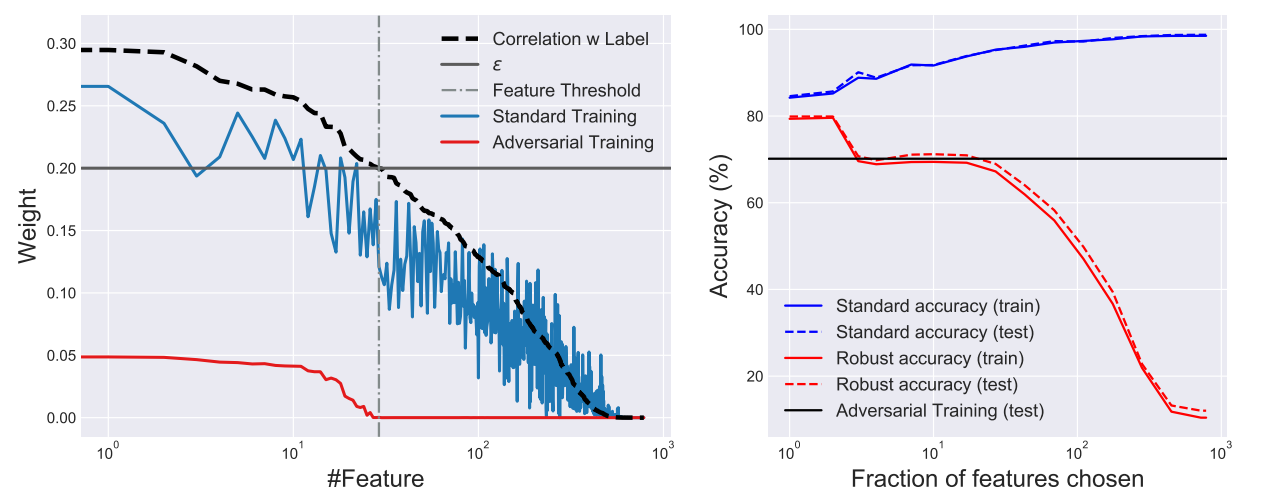
\includegraphics[width=0.8\textwidth]{fig/p2/cu.png}}\\
  Right figure: \\Both accuracy is trained using \textbf{standard} training with subset of features \\
(w/ decreasing relation between label, calculated thru $\mathbb{E}_{(x,y) \sim \mathcal{D}}[yx_i]$)
\end{frame}

%\begin{frame}{Some Lessons}
  %As more features are incorporated into the training, the standard accuracy is improved at the cost of robustness
%\end{frame}


\begin{frame}{Intepretable Gradients: What is robust feature}
  The feature learned during adversarial training is invariant to pertubations.\\
  Loss gradients in the input space align well with human eyes
  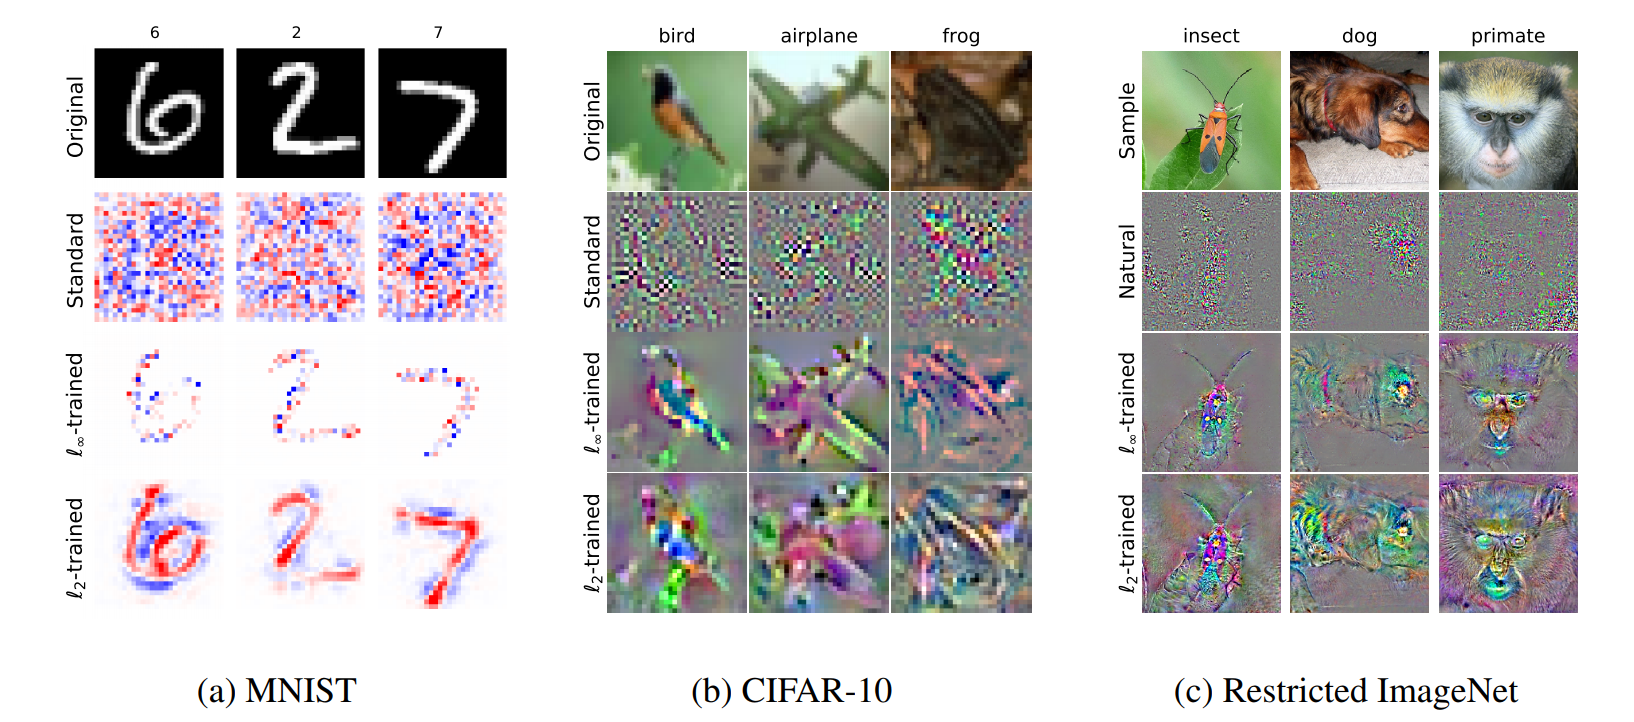
\includegraphics[width=\textwidth]{fig/p2/int-grad.png}
\end{frame}

\begin{frame}{Adversarial Examples: Which input will fool the model}
  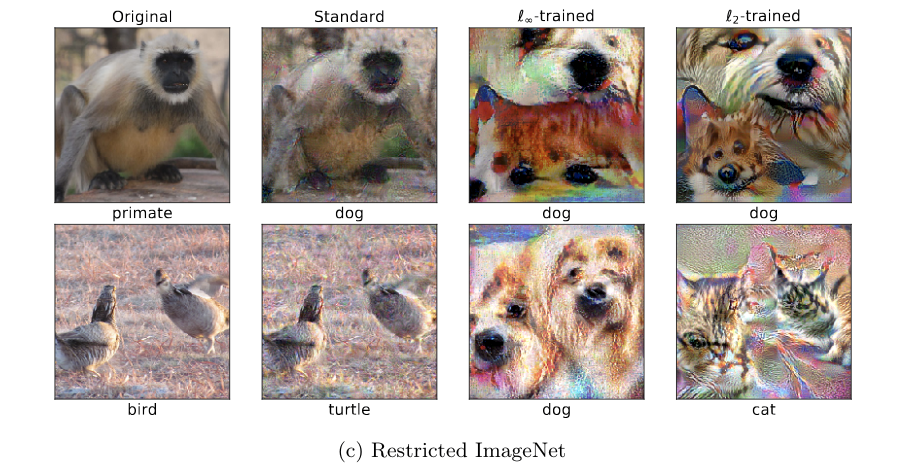
\includegraphics[width=\textwidth]{fig/p2/adv-sample.png}
\end{frame}


\section{Obfuscated Gradients Give a False Sense of Security}
\begin{frame}{Obfuscated Gradients Give a False Sense of Security}
  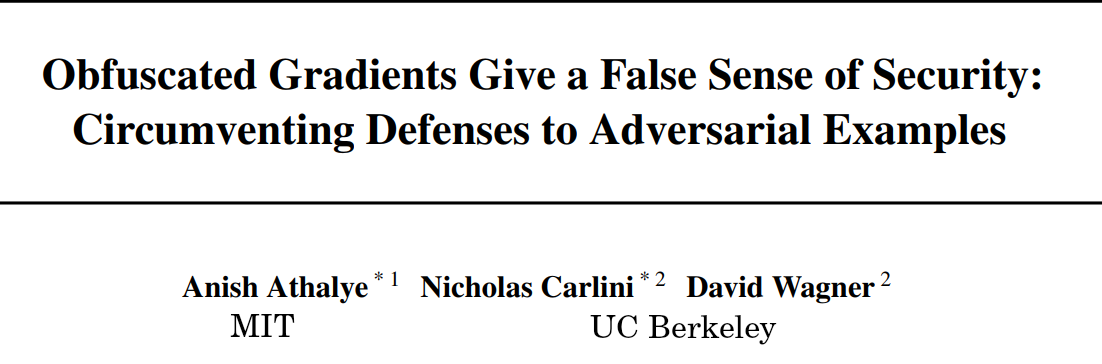
\includegraphics[width=\textwidth]{fig/ob-grad/ob-grad-title.png}
  \center ICML 2018
\end{frame}

\begin{frame}{Some Highlights}
  \begin{itemize}
    \item Provide a method to identify so-called \textbf{Obfuscated Gradients}
    \item Identify 7/9 of defenses proposed in ICLR 2018 succeed defensing by this pheonemon
    \item \textbf{Provide simple algorithms to beat those defenses} \href{https://github.com/anishathalye/obfuscated-gradients}{$\rightarrow$ github}\\
      (within pertubations $\mathcal{S}$ they claim they can defend under white-box setting)
  \end{itemize}
\end{frame}

\begin{frame}{It's Da Lian Time}
  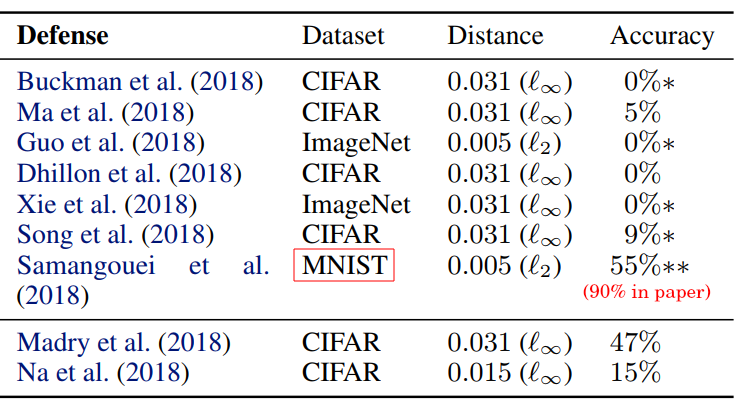
\includegraphics[width=\textwidth]{fig/ob-grad/table.png}
\end{frame}

\begin{frame}{Intuition of Obfuscated Gradients}
  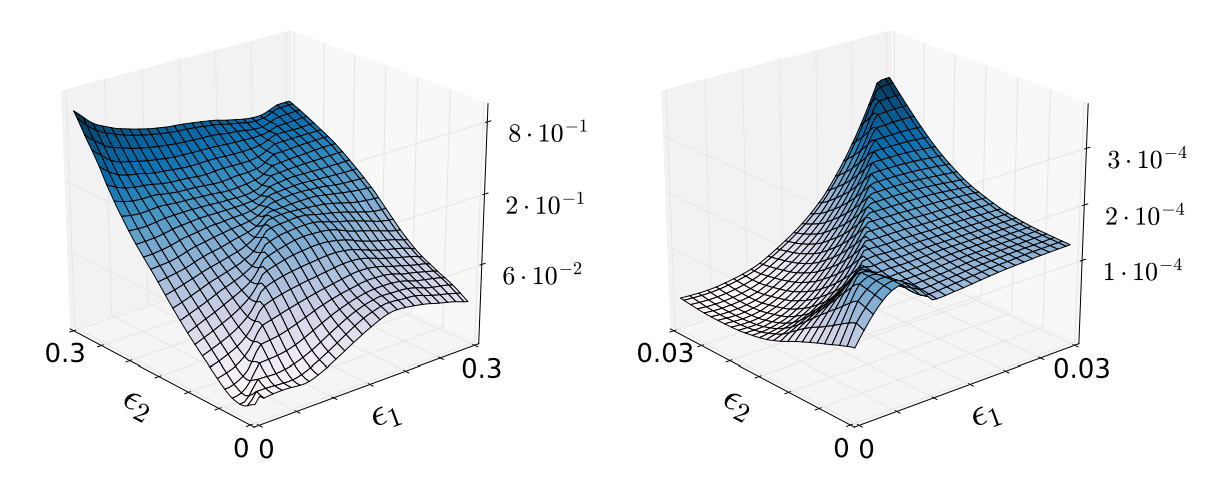
\includegraphics[width=\textwidth]{fig/ob-grad/effect-of-gradient-masking.png}

  %\textbf{Note}: $L(\hat{x},y|\theta)$ is still high within $\mathcal{S}$
\end{frame}

\begin{frame}{How to identify them}
  \begin{itemize}
    \item One-step attacks perform better that iterative attacks
    \item Partial random-step attacks perform better
    \item Black-box attacks perform better (see next slide)
    \item Increasing pertubation budget $\epsilon$ doesn't increase success rate pretty much
  \end{itemize}
\end{frame}

\begin{frame}{Why black-box attack can perform better}
  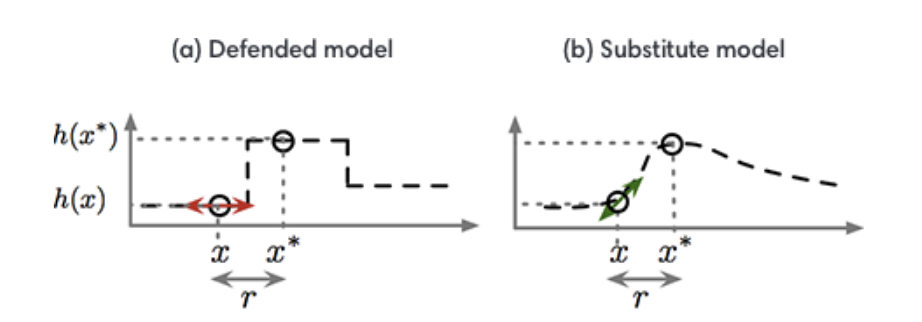
\includegraphics[width=\textwidth]{fig/ob-grad/black-box-attack.png}
\end{frame}

\begin{frame}{Types of Obfuscated Gradients}
  \begin{itemize}
    \item Shattered Gradients 
      \begin{itemize}
        \item non-differentiable operation (\textit{nonexistent})
        \item provide \textit{incorrect} gradient to make adversary stuck in local
      \end{itemize}
    \item Random Gradients
        \begin{itemize}
          \item randomize the network
          \item add some random processing to input
        \end{itemize}
      %\item Exploding/Vanishing Gradients (?)
  \end{itemize}
\end{frame}

\begin{frame}{Proposed Attack Algorithms}
  \begin{itemize}
    \item Backward Pass Differentiable Approximation (\textit{BPDA})
      \begin{itemize}
        \item Circumvent shattered gradients
        \item $\nabla_xf(g(x))|_{x = \hat{x}} \approx \nabla_xf(x)|_{x = g(\hat{x})}$
      \end{itemize}

    \item Expectation over Transformations (\textit{EOT})
      \begin{itemize}
        \item Circumvent random gradients
        \item $\nabla\mathbb{E}_{t \sim T}f(t(x)) = \mathbb{E}_{t \sim T} \nabla f(t(x))$
        \item In brief, ensemble
      \end{itemize}
  \end{itemize}
\end{frame}

\begin{frame}{Some Lesson}
  \begin{itemize}
    \item Succeed attack algorithm can be used as defense algorithm \\
      (thru adversarial training using these samples)
    \item No free lunch, additional cost of
      \begin{itemize}
        \item calculate $g(\cdot)$ many steps
        \item parallel computation cost of ensemble
        \item generalization accuracy (just mentioned before)
      \end{itemize}
  \end{itemize}
\end{frame}
%\begin{frame}{Experiments: Multi-class classification}
  %\center{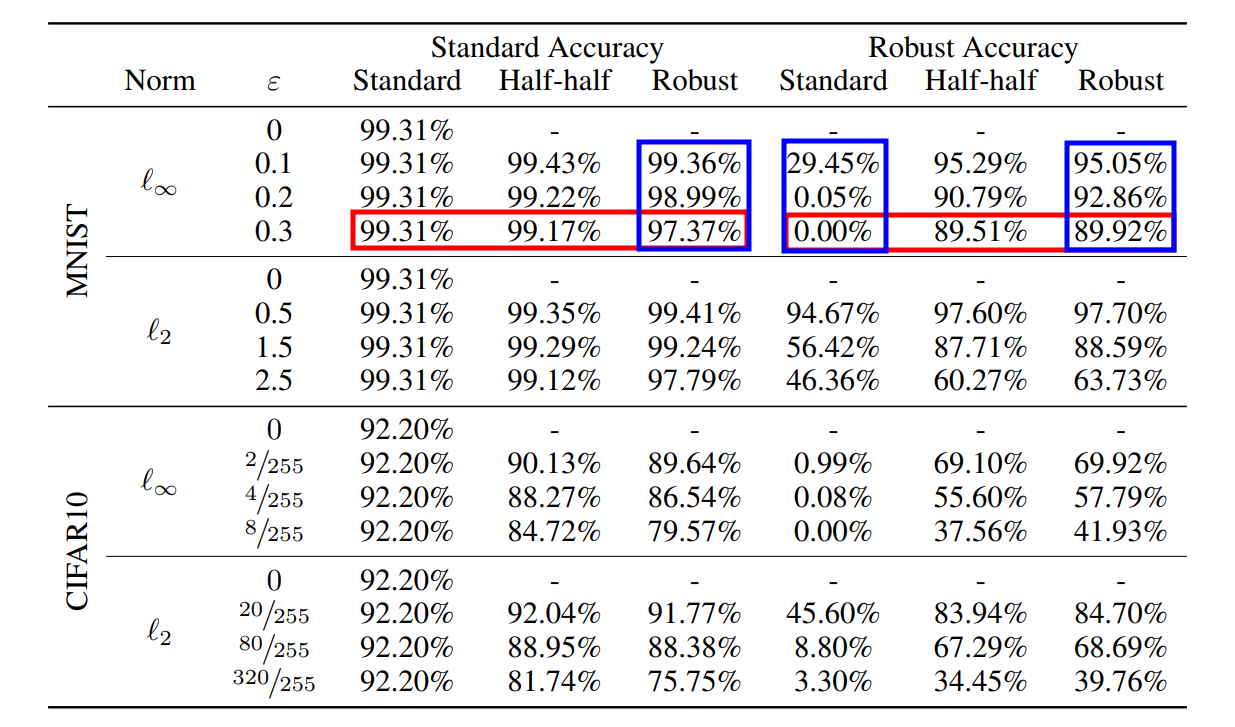
\includegraphics[width=\textwidth]{fig/exp.png}}\\
%\end{frame}


%\section{Other Interesting Aspects}
%\begin{frame}{Other Interesting Aspects}
  %\begin{itemize}
    %\item Transferability of adversarial examples
      %\begin{itemize}
        %\item Intra-technique: That's why black box attack still works well
        %\item Cross-technique: e.g Decision Tree vs NN (even one is differentiable model, one is not)
      %\end{itemize}
    %\item Obfuscated gradients: Over-confidence of adversarial robustness (ICML2018)
  %\end{itemize}
%\end{frame}

\begin{frame}
  \begin{center}
    \weib{\LARGE{謝謝聆聽!}}
    %\LARGE{Questions?}
  \end{center}
\end{frame}




%\begin{frame}{Interpretable gradients}
  %Loss gradients in the input space align well with human eyes
  %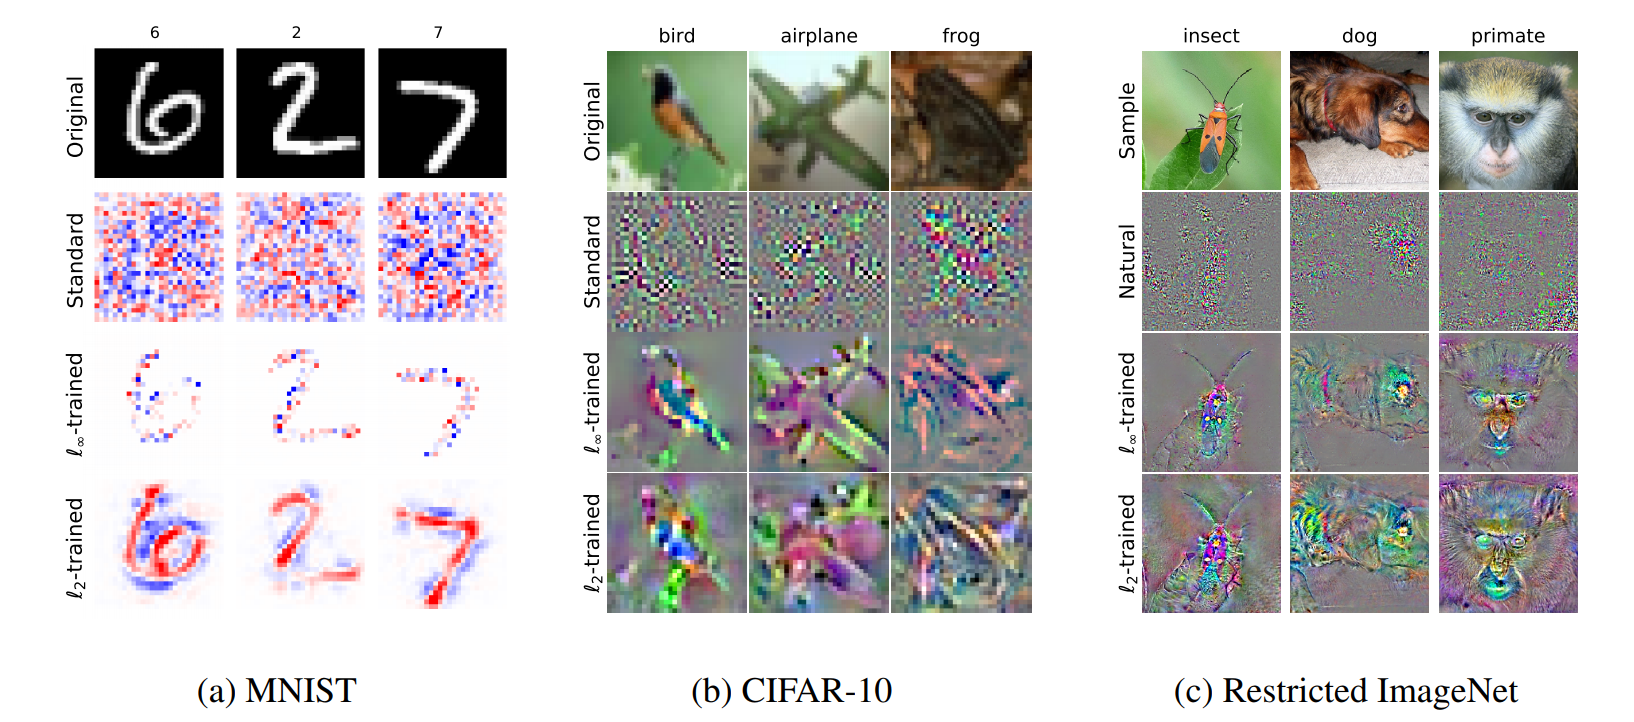
\includegraphics[width=\textwidth]{fig/p2/int-grad.png}
%\end{frame}

%\begin{frame}{Some Thoughts}
  %\begin{itemize}
    %\item By encoding appropriate prior into set of pertubations $\mathcal{S}$, adversarial training can provide interpretable gradients 
  %\end{itemize}
%\end{frame}

\end{document} 
